%section 2 - Status of the IPv4/IPv6 dual-stack transition at WLCG sites
The IPv6 deployment on the Tier-1 storage systems has been completed
and also at Tier-2 sites it has made substantial progress, even if we
are now years past the original deadline at the end of 2018, which was
never officially extended. Many WLCG sites encountered objective
difficulties, very often due to misaligned priorities between the site
and the institute to which it belongs. However, the fraction of sites
having completed the IPv6 deployment on their storage systems is now
93\% and still increasing, as it can be seen in
figure~\ref{fig:t2depl}.

\begin{figure}[h]
\centering
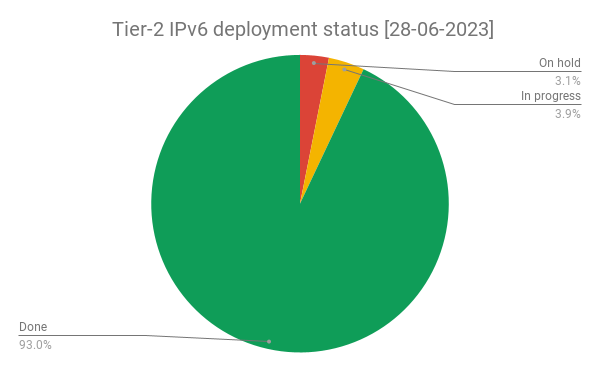
\includegraphics[width=6cm]{chart2}
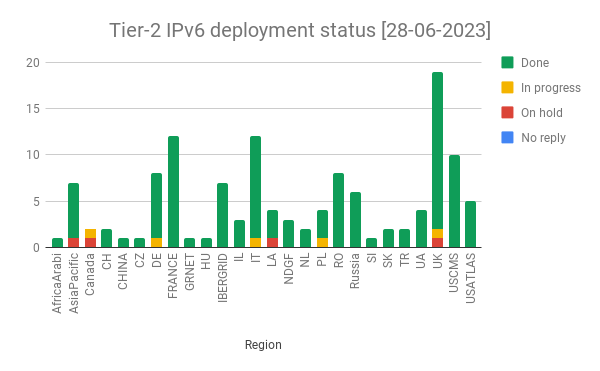
\includegraphics[width=6cm]{chart}
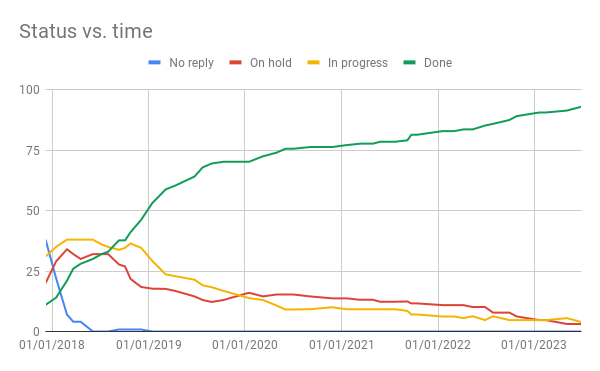
\includegraphics[width=6cm]{chart3}
\caption{(left) Tier-2 deployment status by site globally, (right) by region,
and (bottom) time evolution}
\label{fig:t2depl}
\end{figure}

The fraction of the Tier-2 storage that is accessible via IPv6 is
shown in table~\ref{tab:t012stor} for each experiment; two experiments have
completed the deployment and the other two are in a very good shape.
\begin{table}[h]
\centering
\caption{Fraction of Tier-2 storage available over IPv6}
\label{tab:t12stor}
\begin{tabular}{lccccc}
\hline
& ALICE & ATLAS & CMS & LHCb & Global \\\hline
Tier-2 storage & 91\% & 90\% &  100\% & 100\% & 94\% \\\hline
\end{tabular}
\end{table}

Another important indicator of progress is monitoring, to quantify the level
of adoption of IPv6, for example in data transfers. There are several systems
providing information: perfSONAR, which tests network links between sites
separately for IPv4 and IPv6; ETF, which submits functional tests to site
services, optionally via IPv6; the FTS monitoring, which is supposed to show
which IP version was used for each data transfer, and custom network
utilisation plots, e.g.\ specifically for LHCOPN/LHCONE traffic.

